\documentclass[../thesis.tex]{subfiles}

\begin{document}
\subsection{During Training}\label{subsec:Train}
\begin{figure}[ht]
	\centering
	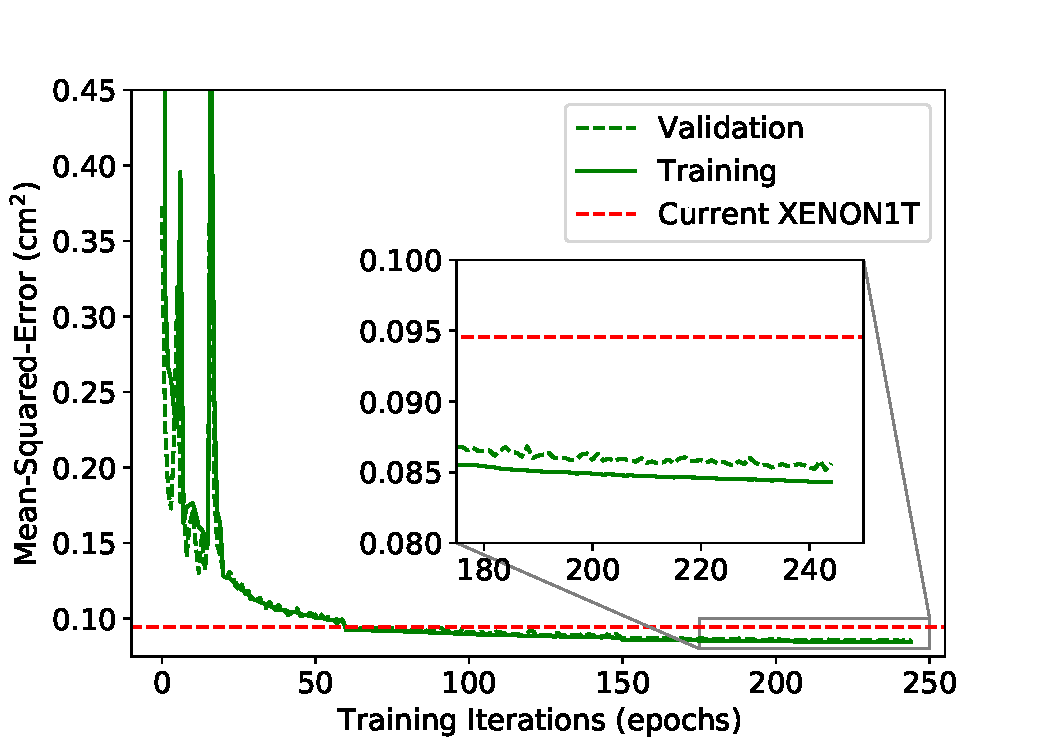
\includegraphics[width=0.8\linewidth]{figures/del_mse-v-epo_insetted.pdf}
	\caption{Mean-Squared-Error (MSE) in square centimeters of our algorithm for the training set and validation set during the training process.
	The minimum MSE for the current state-of-the-art is given in red at 0.0945 cm\textsuperscript{2}.
	This is the benchmark that our algorithm  had to pass during training.
	Spikes within the first 20 epochs occur due to large step size during gradient descent.
	Learning rate was lowered at epochs 20, 60, and 150.
	The minimum MSE achieved by our GCNN on the validation set is 0.0852 cm\textsuperscript{2}.}
	\label{fig:GCNN_Training}
\end{figure}
The performance of our algorithm was compared to the current state-of-the-art in XENON1T during training as a benchmark and early warning system.
If the GCNN did not approach a comparable performance to that of the state-of-the-art swiftly enough, training would typically stagnate and not surpass this benchmark.
By not performing better here, it was generally indicative that the GCNN would also perform worse when we gave attention to our performance metrics.
After a few iterations of this, we chose to only look at the performance metrics if the GCNN model produced a lower mean-squared-error during training and would restart training in cases where it was clear that the current iteration would not perform better within a reasonable number of epochs.
An example of when it was clear a prospective model would not do better is if the mean-squared-error was not below $0.25$ cm\textsuperscript{2} within the first $50$ epochs.
\begin{wrapfigure}{r}{0.5\textwidth}
	\centering
	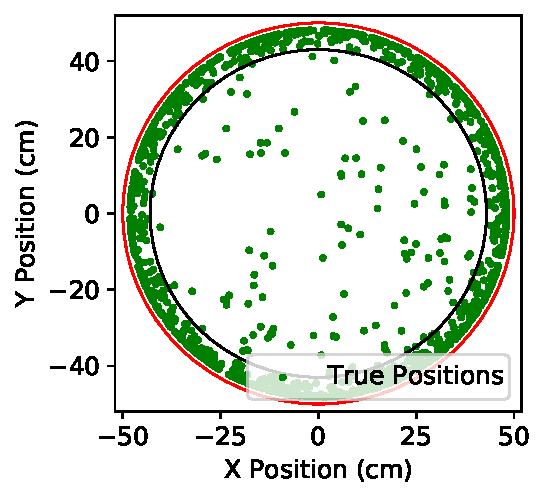
\includegraphics[width=\linewidth]{figures/gcnn_Delaunay-Prenoise_1cm-err.pdf}
	\caption{
	Scatter plot of the true positions of our algorithm's mis-reconstructions.
	The red circle is the wall of the detector (50 cm); the black circle is the largest radius of the fiducial volume (43 cm).
	Of the 197,975 simulated events, there were 1,680 mis-reconstructions which are shown here.
	Within the fiducial volume, there were 123 out of 1,680.
	}
	\label{fig:1cm_Counts}
\end{wrapfigure}

\par We used an optical Monte Carlo simulation of 989,875 events for training as an attempt to assume a “perfect” detector.
This is to say that no spurious events, such as single electrons, dark counts, or PMT after-pulses, were within our simulation.
The observations by the PMTs are as if every part of the detector ran perfectly.
By using a simulation like this, we were able to input the data into our model without normalization or standardization.

\par Our algorithm was able to outperform the state-of-the-art in training, which is a good indicator for the overall performance.
Much of the work for this stage was in optimizing the learning rate used for gradient descent.
Our solution was to lower the learning rate at specific epochs based on the performance of  previous results.
Specifically, the learning rate was lowered at epochs 20, 60, and 150.
This caused notable dips within Figure \ref{fig:GCNN_Training} and resulted in a much smoother curve after epoch 20.
However, a better solution would have the learning rate lower based on the model's performance during training instead of milestones set by the attentive user.

\subsection{Validation Set Performance}\label{subsec:Valid}
As previously stated, the two performance metrics we focused on are to have no reconstructions outside the detector and to minimize the number of reconstructions that are 1 cm away from the true position.
For best practice in machine learning, we focused on the results of the validation set which is made of 197,975 simulated events.
\begin{figure}[t]
	\centering
	\begin{subfigure}[b]{0.45\textwidth}
		\centering
		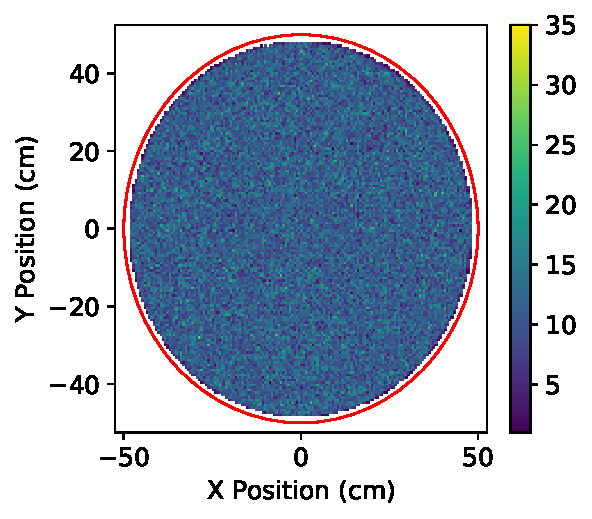
\includegraphics[width=\textwidth]{figures/optsim_val_true_pos.pdf}
	\end{subfigure}
	\hfill
	\begin{subfigure}[b]{0.45\textwidth}
		\centering
		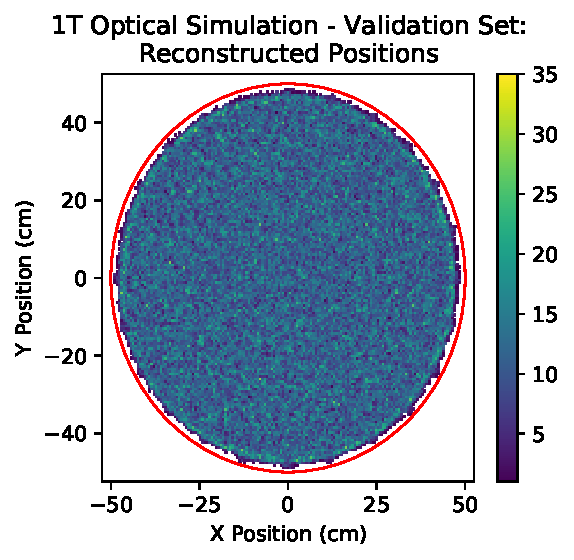
\includegraphics[width=\textwidth]{figures/optsim_val_reco_pos.pdf}
	\end{subfigure}
	\caption{
	2D histograms of the true positions (left) and reconstructed (right) positions at 150 bins.
	Red circle is the wall of the detector (50 cm).
	The edge of the reconstructed positions is noticeably more jagged.
	}
	\label{fig:2D_Hists}
\end{figure}

\par Since we are hard set on having no reconstructions outside of the detector, this was the first metric we would check.
As it turned out, we counted zero reconstructions outside of the detector for our latest version of the GCNN.
At this point, our algorithm has successfully surpassed the state-of-the-art training benchmark and made no exceedingly erroneous reconstructions, a rule that previous implementations had difficulty passing.

\par As for the further than 1 cm reconstructions, these too performed well.
Of the 197,975 events, 1,680 were reconstructed at greater than 1 cm away from the true position, about 0.85\% of the validation set.
As can be seen in Figure \ref{fig:1cm_Counts}, many of the mistakes are made along the walls of the detector and explains the jagged edge found in Figure \ref{fig:2D_Hists}.
If we reduce the area we count on to the maximum radius of the fiducial volume ($R=43$ cm), we find only 123 of the 197,975 events mis-reconstructed, 0.06\% of the validation set.

\par The last important performance check, as for any experiment, is to produce the most accurate measurements or reconstructions, in our case.
For this we use the resolution metrics $\Delta X$, $\Delta Y$, and $\Delta R$:
\begin{gather*}
	\Delta X \equiv X_\text{Reconstructed} - X_\text{Simulated},
	\quad \Delta Y \equiv Y_\text{Reconstructed} - Y_\text{Simulated}, \\
	\quad \Delta R \equiv \sqrt{ \Delta X^2 + \Delta Y^2 }
\end{gather*}
where $X$ and $Y$ are the $x$ and $y$ positions of the reconstructions and the associated simulation.
The means and standard deviations produced by our algorithm are shown in Figure \ref{fig:1D_Hist}.
This too outperformed the state-of-the-art which had standard deviations greater than 3 cm.
From previous observations of the results of our GCNN, the mean and standard deviation of $\Delta R$ follows suit with what we expect: most of the reconstructions are within 1 cm of the true, simulated position.
At the same time, the approximately-Gaussian curves of $\Delta X$, $\Delta Y$, and radius difference further confirms the positive performance of our GCNN.
\begin{figure}[t]
	\centering
	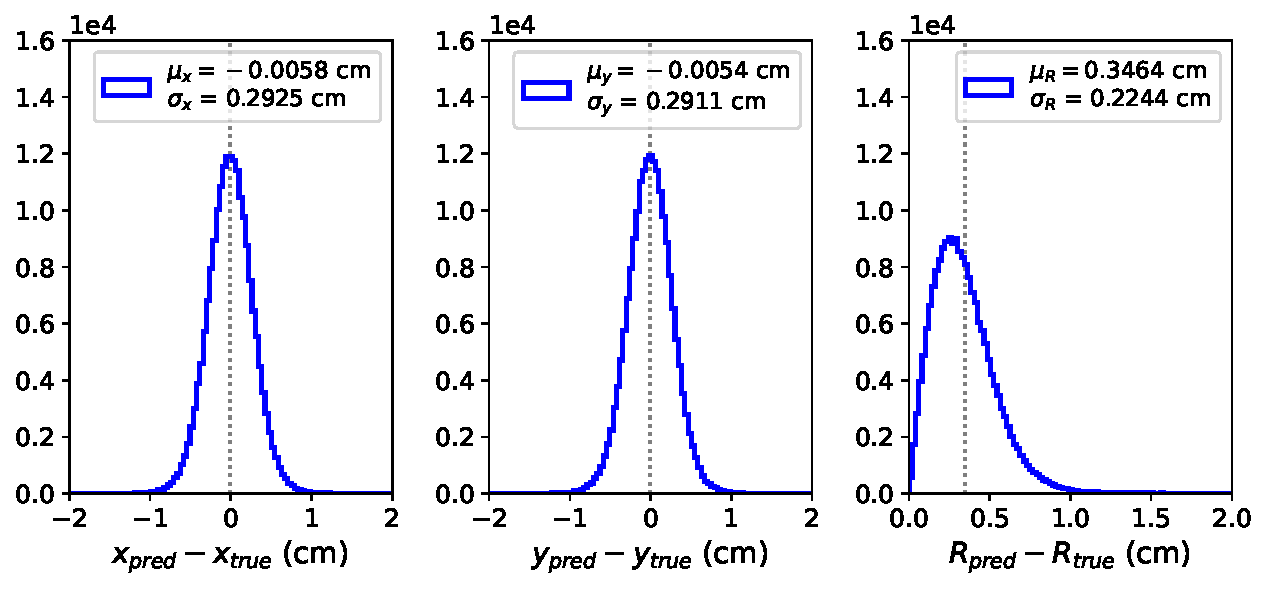
\includegraphics[width=0.9\linewidth]{figures/1D_hist_Delaunay-Prenoise.pdf}
	\caption{
	1D histograms of the reconstructed position minus the true positions.
	There are 100 bins between -2 cm and 2 cm on $\Delta X, \Delta Y, (R_\text{Predicted} - R_\text{True})$ and 100 bins between 0 cm and 3 cm on $\Delta R$.
	The left three histograms are near Gaussian curves of the same statistics.
	}
	\label{fig:1D_Hist}
\end{figure}

\par The visual uniformity of the 2D histogram in Figure \ref{fig:2D_Hists} had us question the true uniformity of both distributions.
We made use of Ripley's $\widehat{K}$ and $\widehat{L}$ functions \cite{Ripley}.
These functions are used for describing spatial uniformity and are defined as:
\begin{align*}
	\widehat{K}(r) &\equiv \dfrac{1}{n\lambda} \sum_{i \neq j} I(d_{ij} < r) \\
	\widehat{L}(r) &\equiv \left( \dfrac{\widehat{K}(r)}{\pi} \right)^{1/2} .
\end{align*}
Here $n$ is the number of points, $\lambda$ is the number of points per unit area, $I(\cdot)$ is an indicator function, $d_{ij}$ is the distance between data points $i$ and $j$.
In the ideal case for perfect, spatial uniformity, $\widehat{K}(r) = \pi r^2$ and $\widehat{L}(r) = r$.

\begin{figure}[t]
	\centering
	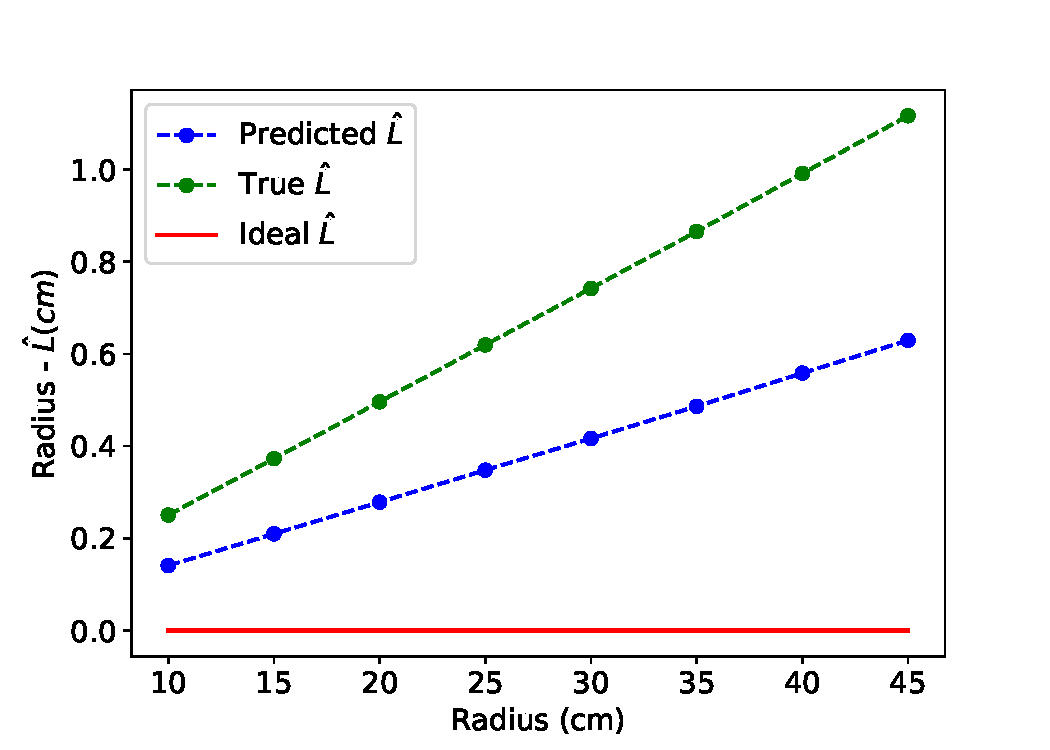
\includegraphics[width=0.8\linewidth]{figures/gcn28_ripley-L.pdf}
	\caption{
	Ripley's $\widehat{L}$ function shifted according to radius.
	The closer to the ideal case is better.
	These values are indicative of a more dispersed set of points.
	}
	\label{fig:Ripley}
\end{figure}

\par The results of applying Ripley's $\widehat{L}$ function are shown in Figure \ref{fig:Ripley} and indicate that the reconstructed positions are more spatially uniform than the true positions.
Both the predicted and true positions are more dispersed than the ideal case, however, these values are not significantly large enough to merit further discussion.

\subsection{Experimental Data}\label{subsec:Experiment}
We applied this trained model to Kr\textsuperscript{83m} data.
However, the detector at that time featured multiple broken PMTs.
Nodes that represent these broken PMTs receive values of 0 instead.
In addition to this, the data is no longer free of background events.
It's expected for the model to do poorly.
One of the first steps we had to do was normalize the data to a similar level that was used during training.
This was done according to:
\begin{equation}
	\hat{x} \propto \dfrac{x}{\sum_{i=1}^{127} x_i}
\end{equation}
where $x$ is the event signal and $\hat{x}$ is the normalized signal.

\begin{figure}[t]
	\centering
	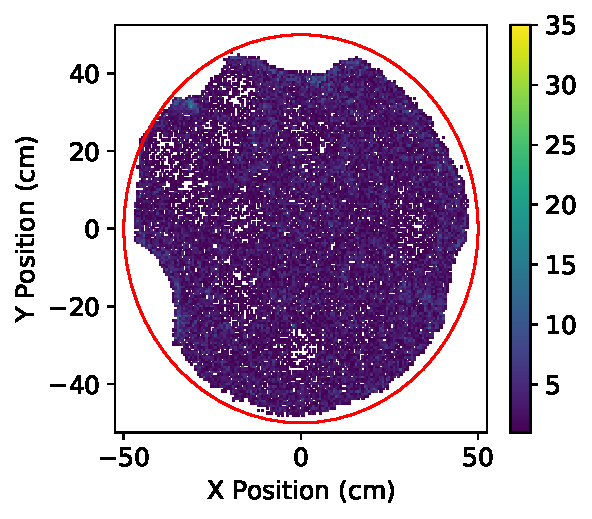
\includegraphics[width=0.5\textwidth]{figures/iso-kr83_reco_pos.pdf}
	\caption{
	2D histogram of the reconstructed positions of Kr\textsuperscript{83m} experimental data.
	The red circle is the wall of the detector (50 cm).
	The low density areas and inward curves along the edge the histogram are the same positions as the broken PMTs.
	}
	\label{fig:iso_2D-hist}
\end{figure}

\par The result of the model on normalized, experimental data is better than we expected.
The low density areas and inward curves along the edge of the reconstructions in Figure \ref{fig:iso_2D-hist} occurs in the same positions as the broken PMTs.
The effect of 0 values at the associated nodes indicates that events would not take place under those nodes and should therefore be reconstructed elsewhere.
Although this result is not useful for position reconstruction, this does indicate the model is able to learn the detector.
Another notable result is the limited number of events that are reconstructed outside of the detector.
For a model that was trained on a ``perfect'' detector, these results are much better and more meaningful than expected.

\end{document}
